\documentclass{article}
\usepackage{graphicx,fancyhdr,amsmath,amssymb,amsthm,subfig,url,hyperref}
\usepackage[margin=1in]{geometry}
\usepackage{xltxtra}
\usepackage{xgreek}
\usepackage{amsfonts}
\usepackage{amssymb}
\usepackage{amsmath}
\usepackage{graphicx}
\usepackage{caption}

%\setmainfont[Mapping=tex-text]{Times New Roman}
\setmainfont{GFS Artemisia}
%----------------------- Macros and Definitions --------------------------
% FILL THIS OUT
\newcommand{\studentname}{Νικόλαος Ζαρίφης}
\newcommand{\suid}{03112178}
\newcommand{\exerciseset}{Δεύτερη εργαστηριακή Άσκηση}
% END



\renewcommand{\theenumi}{\bf \Alph{enumi}}

%\theoremstyle{plain}
%\newtheorem{theorem}{Theorem}
%\newtheorem{lemma}[theorem]{Lemma}

\fancypagestyle{plain}{}
\pagestyle{fancy}
\fancyhf{}
\fancyhead[RO,LE]{\bfseries\large NTUAthens}
\fancyhead[LO,RE]{\bfseries\large Δίκτυα επικοινωνιών}
\fancyfoot[LO,RE]{\bfseries\large \studentname: nick.zarifis@hotmail.com}
\fancyfoot[RO,LE]{\bfseries\thepage}
\renewcommand{\headrulewidth}{1pt}
\renewcommand{\footrulewidth}{1pt}

\graphicspath{{figures/}}

%-------------------------------- Title ----------------------------------

\title{Δίκτυα επικοινωνιών \\ \exerciseset}
\author{\studentname \qquad  ID: \suid}

%--------------------------------- Text ----------------------------------

\begin{document}
\maketitle

\section*{Problem 1}
\begin{enumerate}
\item []
Στην πρώτη προσομοίωση βλέπω πως τα πακέτα μετά το 1.65 ξεκινάνε να χάνονται αυτό συμβαίνει γιατί: Η γραμμή που ενώνει τους κόμβους 2 και 3 αντέχει κάθε στιγμή $2Mbits * 10ms=2*10^4bis \rightarrow 0.25*10^4bytes$ Τώρα από τον κόμβο 0
έρχονται max $1000*\frac{10ms}{5ms}=2000bytes$ . Και από τον κόμβο 1 :$1000*\frac{10ms}{8ms}=1.25*1000bytes$. Άρα συνολικά:
$3.25*10^3=0.325*10^4>0.25*10^4$ άρα τα νέα πακέτα θα χάνονται. \\
\begin{figure}[ht!]
	\centering
	\subfloat[DropTail]{
		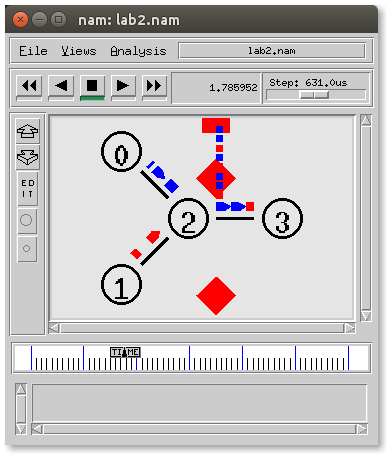
\includegraphics[height=150pt,width=150pt]{drop1}
	}	\subfloat[SFQ]{
	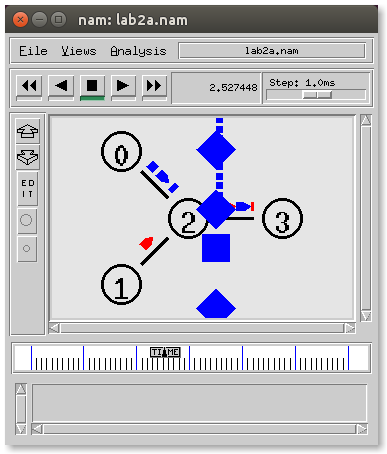
\includegraphics[height=150pt,width=150pt]{sfq}
}
\end{figure}
\end{enumerate}
\title{\textbullet{Ερωτήσεις 1.6}}
\begin{enumerate}
\item   
\begin{figure}[ht!]
	\centering
	\subfloat[DropTail]{
		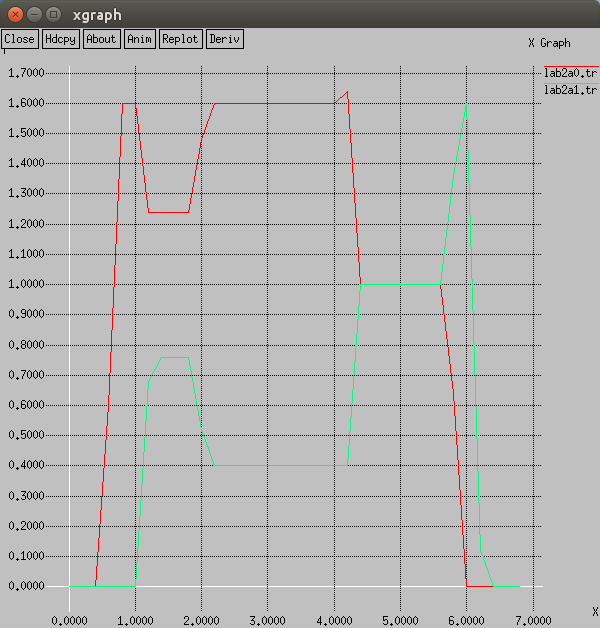
\includegraphics[height=150pt,width=150pt]{xgraphDrop}
	}	\subfloat[SFQ]{
	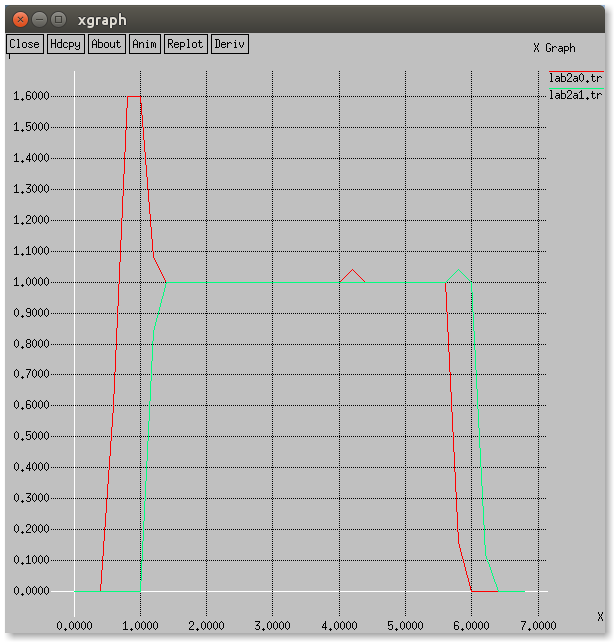
\includegraphics[height=150pt,width=150pt]{xgraphSFQ}
}
\end{figure}
Βλέπουμε ότι στην περίπτωση του DropTail έχουμε στον κόμβο 0 μέγιστη ταχύτητα 1,64Mbs ενώ στον 1 έχουμε 1.6Mbs.
Τώρα όταν έχουμε SFQ ο κόμβος 0 έχει 1.6Mbs και ο 1 1,04Mbs.
\item
Όταν έχουμε DropTail ο κόμβος 0 έχει ελάχιστο 1Mbs ενώ ο κόμβος 1 έχει 0.4Mbs.Αλλά όταν έχουμε SFQ το ελάχιστον κι στους 2 κόμβους έιναι 1Mbs.
\item 
Για να βρούμε τα μέγιστα ποσόστα κάνουμε $\frac{Max-Min}{Max}$.
Έτσι έχουμε για DropTail:\\ Στον Κόμβο 0 $\frac{1.64-1}{1.64}=0.3902\rightarrow 39\%$  Και στον Κόμβο 1: $\frac{1.6-0.4}{1.6}=0.75\rightarrow 75\%$ .Οι μέγιστες απώλειες είναι 0.64Mbs και 1.2Mbs αντίστοιχα.\\
Για SFQ:\\
 Στον Κόμβο 0 $\frac{1.6-1}{1.6}=0.375\rightarrow 37.5\%$  Και στον Κόμβο 1: $\frac{1.04-1}{1.04}=0.038\rightarrow 3.8\%$ .Οι μέγιστες απώλειες είναι 0.64Mbs και 0.04Mbs αντίστοιχα.
\item
Στο animation βλέπουμε ότι χάνονται μόνο μπλε πακέτα όποτε μεταφέρονται όλα τα κόκκινα πακέτα κι μεταφέρονται όσα μπλε χωράνε στην ζεύξη.Άρα 1Mbs μένει για μπλε πακέτα, όμως σύμφωνα με παραπάνω περισσεύουν 0.6Mbs που αυτά χάνονται.Δηλαδή: $\frac{1.6-1}{1.6}=0.375\rightarrow37.5\%$ απώλειες. 
\item
Σύμφωνα με τις προηγούμενες μετρήσεις μας έχουμε ότι η γραμμή αντέχει 2.500Β και έρχονται 3250Β .Άρα χάνονται $\frac{3.250-2.500}{3.250}=0.23$ δηλαδή 23\% .Από τα ποσοστά που βρήκαμε πριν έχουμε για Droptail: Έχουμε ότι στέλνουμε απο τον 0 , 2000Bytes άρα έχουμε απώλειες $2000*0,39=780Bytes$ και κόμβο 1: $1000*0,75=750Bytes$ συνολικά: 1530Bytes>750Bytes που ήταν το αναμενόμενο.

Και για SFQ: Στον κόμβο 0 έχουμε: $2000*0,375=750Bytes$ και κόμβο 1: $1000*0,038=38Bytes$ συνολικά: 788Bytes>750Bytes.
Αυτό γίνεται γιατί η ούρα τύπου DropTail είναι FIFO άρα αφού έρχονται πιο συχνά μπλε πακέτα αποκρύπτονται τα κόκκινα.Έτσι βλέπουμε ότι η ουρά τύπου SFQ είναι πιο κοντά στις θεωρητικές απώλειες.
\item
Τα διαστήματα μηδενικής κυκλοφορίας είναι όταν στην γραμμή δεν έχει φτάσει ακόμα κανένα πακέτο ή όταν έχει τελειώσει η μεταφορά.Παρατηρούμε ότι όταν έχουμε droptail ο ρυθμός μετάδοσεις ξεπερνά αυτόν της πηγής. Πράγμα που γίνεται γιατί στην ουρά έχουμε πάκετα έτοιμα να φύγουν κι δεν ακολουθούν έτσι την ταχήτατα που τα στέλνει η πηγή.
\end{enumerate}
\section*{Problem 2}
\begin{enumerate}
\item %A
Θέλοντας να στείλουμε από τον κόμβο 0 στον κόμβο 4, το δίκτυο όπως είναι λογικό  ψάχνει την συντομότερη διαδρομή στην αρχή.Έπειτα στέλνει πακέτα μέχρι το 1.5 όπου πέφτει η γραμμή που ενώνει τον κόμβο 3 μέ 4 και έτσι το ψάχνει να βρει μια εναλλάκτη διαδρομή που να λειτουργεί ώστε να στείλει τα υπόλοιπα πακέτα,έπειτα όταν ξανά-ανέβει η ακμή το δίκτυο ξεκινά πάλι να στέλνει από την συντομότερη διαδρομή.Αυτό επιτυγχάνεται με τα rtprotoDV όπου έχουν πληροφορίες σχετικά με την σύνδεση των κόμβων που συνδέουμε .  
\item
Αυτό συμβαίνει γιατί ακόμα δεν έχει ενημερωθεί ο κόμβος για το ότι έπεσε η γραμμή κι δεν έχει φτάσει ακόμα το πακέτο που το ενημερώνει κι του δίνει την νέα διαδρομή για να στείλει.
\item
Αυτό συμβαίνει γιατί τα πακέτα rtprotoDV λένε ότι εκεί μπορεί να συνεχιστεί η σύνδεση με την μικρότερη απόσταση.(αν κι εδώ είναι η μοναδική εναλλακτική διαδρομή.)
\end{enumerate}
\begin{enumerate}
\begin{figure}[ht!]
	\centering
	\subfloat[time:$0.2$]{
		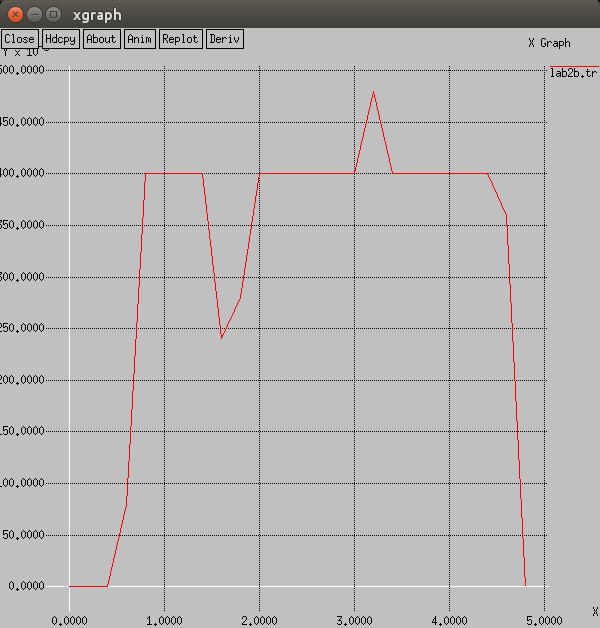
\includegraphics[height=150pt,width=150pt]{xgraph2}
	}	\subfloat[time: $0.08$]{
	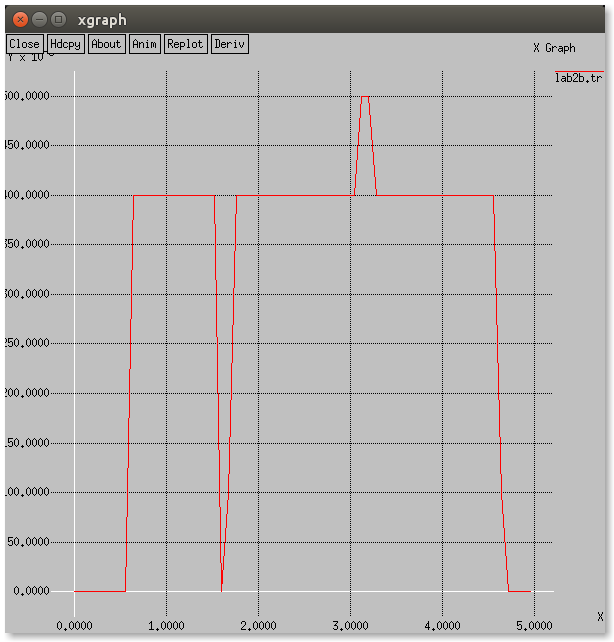
\includegraphics[height=150pt,width=150pt]{xgraph008}} 
	\subfloat[time: $0.02$]{
		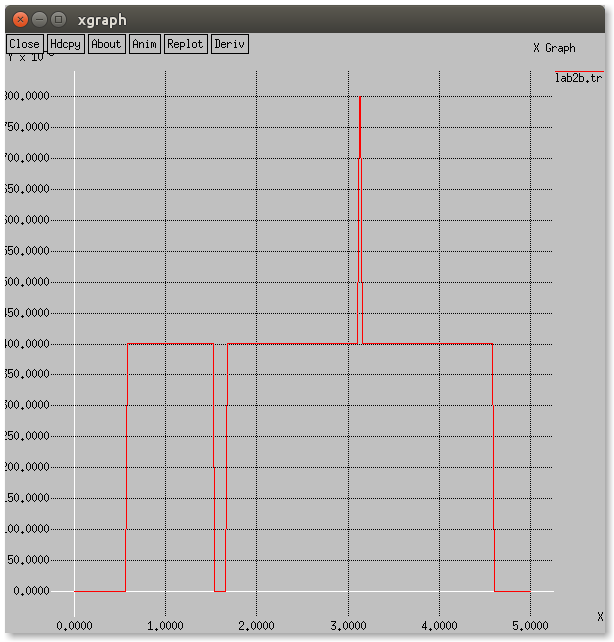
\includegraphics[height=150pt,width=150pt]{xgraph002}}


\end{figure}
\item
Το γράφημα δεν είναι σωστό γιατί από το 1.5 μέχρι να βρει την νέα διαδρομή έπρεπε να μηδενίζεται πράγμα που δεν γίνεται εδώ. Βέβαια είναι αναμενόμενο με τόσο υψηλό time που έχουμε στο record.
\item
Αλλάζοντας το time του record βλέπουμε στα σχήματα (β'),(γ') ότι η γραφική γίνεται όλο κι πιο ακριβής .
\item
Στην τελευταία γραφική παράσταση βλέπουμε ότι φτάνει στα 0.8Mbs κι αυτό είναι λογικό γιατί εκείνη την στιγμή στέλνονται πακέτα από 2 διαδρομές κι αφού η έχουμε μέγιστη ταχύτητα 0.4Mbs αιτιολογείται το αποτέλεσμα.

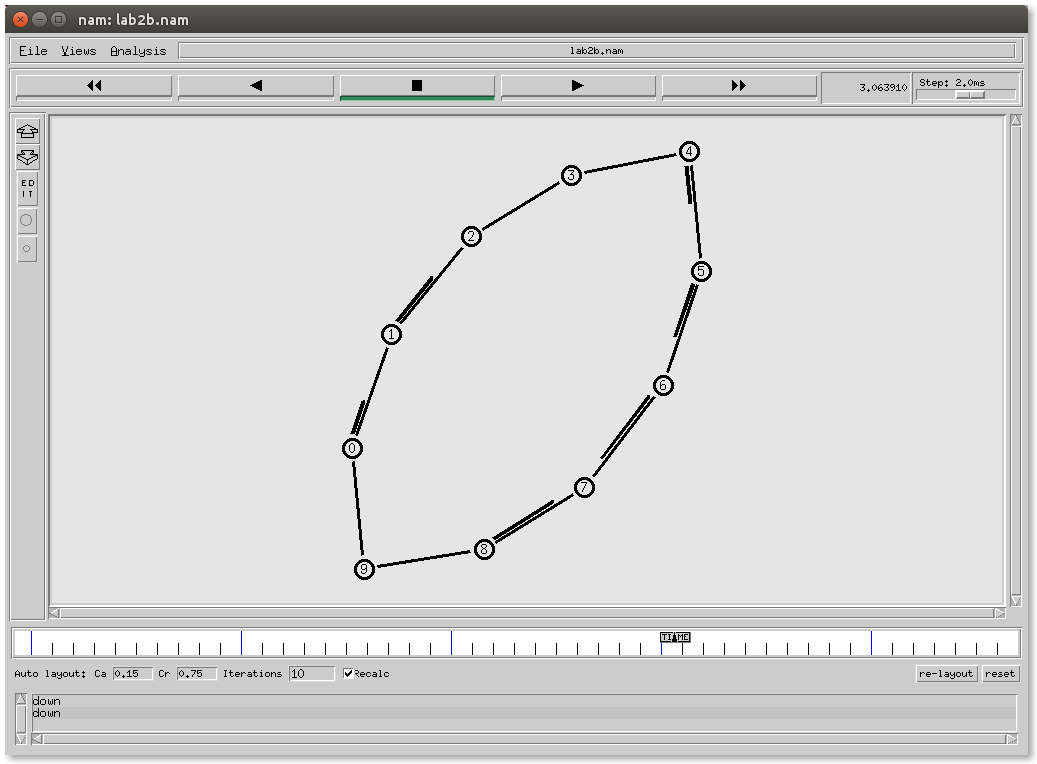
\includegraphics[height=150pt,width=150pt]{nam}
\item
Βλέποντας την γραφική , μέχρι τα 0.5 δεν στέλνονται πακέτα πάρα μόνο τα rtprotoDV , και έπειτα ξεκινάνε να στέλνονται πακέτα μέχρι το μέγιστο 0.4Mbs.Παραμένει σταθερή η εκεί, ως ότου πέφτει η γραμμή 3-4 , γιαυτό πάει στο 0 η γραφική, και έπειτα με το που βρει την νέα διαδρομή ξεκινά να στέλνει πακέτα μέχρι σταθερά στα 0.4Mbs .Όταν ανέβει πάλι γραμμή 3-4 τότε για ένα μικρό χρονικό διάστημα στέλνονται πακέτα κι από τις δύο μεριές , γιαυτό το λόγο η διπλασιάζεται ο ρυθμός. Κι τέλος μένει σταθερή ακόμα στα 0.4Mbs μέχρι το τέλος.
\end{enumerate}

\end{document}